\documentclass[floatsintext, 11pt, doc]{apa6}

%\usepackage{gb4e}
%\usepackage{pslatex}
\usepackage{apacite}
\usepackage{amsmath,amssymb}
%\usepackage[super, numbers]{natbib}
\usepackage{graphicx}
\usepackage{color}
\usepackage{url}
\usepackage{fullpage}
\usepackage{setspace}
\usepackage{booktabs}
\usepackage{lingmacros}
\linespread{1.2}
%\newcommand{\url}[1]{$#1$}

\definecolor{Blue}{RGB}{50,50,200}
\newcommand{\blue}[1]{\textcolor{Blue}{#1}}

\definecolor{Red}{RGB}{255,0,0}
\newcommand{\red}[1]{\textcolor{Red}{#1}}

\definecolor{Green}{RGB}{50,200,50}
\newcommand{\ndg}[1]{\textcolor{Green}{[ndg: #1]}}  

\definecolor{blueish}{RGB}{20,150,250}
\newcommand{\blueish}[1]{\textcolor{blueish}{#1}}
\newcommand{\mht}[1]{\textcolor{blueish}{[mht: #1]}}  


 \newcommand{\denote}[1]{\mbox{ $[\![ #1 ]\!]$}}

\newcommand{\subsubsubsection}[1]{{\em #1}}
\newcommand{\eref}[1]{(\ref{#1})}
\newcommand{\tableref}[1]{Table \ref{#1}}
\newcommand{\figref}[1]{Figure \ref{#1}}
\newcommand{\appref}[1]{Appendix \ref{#1}}
\newcommand{\sectionref}[1]{Section \ref{#1}}


% these packages are needed to insert results 
% obtained from R into the LaTeX document
\usepackage{pgfplotstable}
\usepackage{csvsimple}
\usepackage{siunitx}

% set the name of the folder in which the CSV files with 
% information from R is stored
\newcommand{\datafoldername}{csv_data_4_tex}

% the following code defines the convenience functions
% as described in the main text below

% rlgetvalue returns whatever is the in cell of the CSV file
% be it string or number; it does not format anything
\newcommand{\rlgetvalue}[4]{\csvreader[filter strcmp={\mykey}{#3},
             late after line = {{,}\ }, late after last line = {{}}]
            {\datafoldername/#1}{#2=\mykey,#4=\myvalue}{\myvalue}}

% rlgetvariable is a shortcut for a specific CSV file (myvars.csv) in which
% individual variables that do not belong to a larger chunk can be stored
\newcommand{\rlgetvariable}[1]{\csvreader[]{\datafoldername/myvars.csv}{#1=\myvar}{\myvar}\xspace}

% rlnum format a decimal number
\newcommand{\rlnum}[2]{\num[output-decimal-marker={.},
                             exponent-product = \cdot,
                             round-mode=places,
                             round-precision=#2,
                             group-digits=false]{#1}}

\newcommand{\rlnumsci}[2]{\num[output-decimal-marker={.},
                          scientific-notation = true,
                             exponent-product = \cdot,
                             round-mode=places,
                             round-precision=#2,
                             group-digits=false]{#1}}

\newcommand{\rlgetnum}[5]{\csvreader[filter strcmp={\mykey}{#3},
             late after line = {{,}\ }, late after last line = {{}}]
            {\datafoldername/#1}{#2=\mykey,#4=\myvalue}{\rlnum{\myvalue}{#5}}}

\newcommand{\rlgetnumsci}[5]{\csvreader[filter strcmp={\mykey}{#3},
             late after line = {{,}\ }, late after last line = {{}}]
            {\datafoldername/#1}{#2=\mykey,#4=\myvalue}{\rlnumsci{\myvalue}{#5}}}

\newcommand{\betaCI}[2]{
 \(\beta = \rlgetnum{#1}{Rowname}{#2}{Estimate}{2}\) ($\rlgetnum{#1}{Rowname}{#2}{l.95..CI}{2}$, $\rlgetnum{#1}{Rowname}{#2}{u.95..CI}{2}$)
}

%\newcommand{\bb}[1]{\mathbb{#1}}
 
% ggplot colors: "#F8766D", "#A3A500", "#00BF7D", "#E76BF3", "#00B0F6"

% variations on blue: "#007fb1", "#4ecdff"


%% TODO
% somewhere in the intro, discuss what other theories of scalar implicature/utterance interpretation have to say about world knowledge 
% add Exp. 4 (run it first...)
% rework discussion
% add appendix with all items

% in intro (or discussion?) talk about what other people have said about how world knowledge is integrated in utterance interpretation, and data that shows that it does. e.g., from guerts (2010, p. 78) : "In general, a sentence like ÒThe peanut was in loveÓ, would yield a massive N400 for the last word. But what will happen when this sentence is embedded in a discourse like the following: 'A woman saw a dancing peanut who had a big smile on his face. The peanut was singing about a girl he had just met. And judging from the song, the peanut was totally crazy about her. The woman thought it was really cute to see the peanut singing and dancing like that. The peanut was {salted/in love}, and by the sound of it, this was definitely mutual. He was seeing a little almond.' (Nieuwland and van Berkum 2006: 1106) As reported by Nieuwland and van Berkum, in this context it is ÒsaltedÓ, not Òin loveÓ, that elicits an N400. Apparently, the expectations tracked by the N400 take into account contextual information, as well as general world knowledge. One of the most salient components of the context is the speaker, and van Berkum et al. (2008) showed that the N400 takes into account information about the speaker, too. In van Berkum et al.Õs study, people listened to sen- tences whose meanings might be at odds with reasonable assumptions about the speakerÕs sex, age, or social status, as inferred from the speakerÕs voice. For example, when ÒI have a large tattoo on my backÓ was spoken in an upper- class accent, there was an obvious discrepancy between social elevation and dorsal decoration, which became apparent at the critical word ÒtattooÓ. This type of mismatch, too, turned out to yield an N400."

\title{Probabilistic beliefs mediate the influence of intuitive theories on generic language}
  \author{Michael Henry Tessler\textsuperscript{1}~\& Noah D. Goodman\textsuperscript{2}}
\affiliation{
\vspace{0.5cm}
 \textsuperscript{1} Massachusetts Institute of Technology, Department of Brain and Cognitive Sciences\\\textsuperscript{2} Stanford University, Departments of Psychology and Computer Science 
}

\begin{document}

\maketitle

\begin{abstract}

Human knowledge about categories is expressed in generic language (, or generics; e.g., ``Birds have hollow bones''). 
Generics are rife with puzzling statistical properties and paradoxes, which many have taken as evidence that generics express some kind of special mental relationship between an abstract kind and its properties rather than a probabilistic relationship. 
\citeA{Tessler2019} formalize a meaning for generics without appealing to special mental relationships but instead draw upon distributional knowledge about properties and principles of Bayesian belief-updating.
Under this model, intuitive theories can influence understanding of generic language by two statistical avenues: knowledge of a property among other categories and predictive beliefs about the future. 
Here we re-examine two key data-points that purport to show that intuitive theories modulate understanding of generics without influencing statistical knowledge. 
Contra the original conclusions, we find the relevant empirical signatures are predicted by a model with no special mental relationship that a generic picks out, but instead general principles of structured probabilistic models of human cognition. 
We argue that a Bayesian framework for intuitive theories have the appropriate mechanisms to influence generic language understanding without generics having to refer to a special mental relationship.

\textbf{Keywords:} 
intuitive theories; generic language; semantics; pragmatics
\end{abstract}

\section{Introduction}
\label{sec:intro}


Generic language (or, \emph{generics}, e.g., ``Alligators have big teeth'') convey generalizable information about categories \cite{Carlson1977, Carlson1995}.
Generics are believed to be a part of every human language \cite{Behrens2005}, are understood by children as soon as they have the syntactic knowledge to combine a subject and a predicate \cite{graham2011two}, and guide the development of intuitive theories \cite{Gelman2003}.
Despite being morphosyntactically simple and ubiquitous in political, scientific, and everyday discourse, generics are rife with statistical paradoxes and puzzles.
For instance, ``Robins lay eggs'' is a true generic, while ``Robins are female'' sounds odd to most people: yet, in both cases, only roughly 50\% of the category has the property (i.e., the female birds). 
The standard generalization drawn from this and many other examples is to say that generics are not statements of statistical information \emph{per se}; instead, many argue, generics convey special mental relationships between kinds and properties \cite{Gelman2007, Leslie2008, Prasada2000, Cimpian2010theory, Cimpian2010}.

The rules that govern special mental relationships between kinds and properties are often correlated with statistical information, but they are separable from statistical knowledge in deep ways that reflect the hidden structure of human thought.
For example, some generics communicate about properties that are relatively enduring in a category \cite{Lyons1977, Prasada2006}, and these generics are somewhat resilient to counterexamples (e.g., the existence of three-legged-dogs does not falsify the generic ``Dogs have four legs'').
Consistent with this intuition, \citeA{Gelman2007} found that adults endorse generics about novel categories like ``Dobles have claws'' irrespective of how many dobles have claws at this present moment, if the way in which dobles acquire claws is genetically determined, as opposed to acquiring them through their environment.
Another feature of intuitive theories that is thought to directly relate to generic language is the status of the property as \emph{striking}, \emph{alarming}, or \emph{dangerous}, wherein people accept generics about dangerousness properties, even when the actual prevalence of the feature within the category is low (e.g., the number of mosquitos that carry the West Nile Virus is exceedingly small but ``Mosquitos carry West Nile Virus'' is true; \citeNP{Leslie2007}). 
Consistent with this viewpoint, \citeA{Cimpian2010} found participants willing to endorse generics about striking properties (e.g., ``Lorches have dangerous feathers'') more so than that of neutral properties (e.g., ``Lorches have purple feathers'') at low levels of prevalence (e.g., when only 30\% of the category have the property).

Recent work in probabilistic models of language understanding, however, has shown that many of the standard ``paradoxes'' of generic language can be resolved without appealing to special mental relationships, but instead drawing upon distributional knowledge about properties and principles of Bayesian belief-updating.
A simple, quantificational semantic theory for generics---generics convey that a relatively high percentage of the category has the property---can account for human judgments of generics across different dependent measures; the key insight is that what counts as \emph{relatively high} depends upon a listener's prior beliefs about the property and where what gets communicate is a speaker's predictive beliefs about the category, not the raw empirical frequencies \cite{Tessler2019}. %, TesslerGenIntMS}.
For example, ``Robins lay eggs'' is intuitively true while ``Robins are female'' is not because laying eggs is a feature that distinguishes robins from many other animals, while the property of being female is present in almost all animal categories in exactly the same proportion.
Under this model, there are two natural avenues through which intuitive theories could influence understanding of generic language: knowledge of a property among other categories and predictive beliefs about the future. 

We re-examine the two key data points arguing for the special mental relationships view: one concerning \emph{property origins} \cite{Gelman2007} and one concerning \emph{property strikingness} \cite{Cimpian2010}.% that argue for the role of special mental relationships in the meaning of generics. 
We replicate the original behavioral patterns, while also measuring the relevant probabilistic constructs that are predicted by \citeA{Tessler2019} to be the intermediate representation between intuitive theories and generic language. 
We find that knowledge about the origins of a property changes human expectations about the prevalence of the property among future members of the category in the exact way that the probabilistic model of generic language would predict given the influence of property origins on generic language.
Additionally, we find that knowledge about the strikingness or dangerousness properties changes listeners' prior expectations about the property in a way that makes dangerous properties seem more distinctive, and thus make generics acceptable even when the property is not very common.
Thus, probabilistic knowledge mediates the influence of intuitive theories on generic languages, consistent with Bayesian approaches to intuitive theories. 


\section{Results}

We examine two case studies that purport to show that generics convey special mental relationships between kinds and properties through the lens of a probabilistic model of generic language, in which no such special relationships exist. 
The first experiment highlights that the origins of a property---how instances of the kind came to have the property---plays a role in the endorsement of generic sentences such as ``Dobles have claws''.
The second shows how the strikingness or dangerousness of properties can also impact endorsements of generic sentences.
We re-examine each of these findings in turn. 

\subsection{Experiment 1: Property origins}

The original paradigm by \citeA{Gelman2007} introduced participants to a novel categories (\emph{dobles}) through a picture book, which also conveyed how instances of the category came to have a property (\emph{property origins}) as well as whether or not they maintained the property throughout their lives (\emph{outcome}).
Participants saw either that the creatures were born with the feature (\emph{intrinsic origins}, e.g., dobles are hatched out of the egg with claws) or acquired it through experience (\emph{extrinsic origins, e.g., dobles find claws on the ground and put them on}) and then either maintain or lose the property following an event (\emph{lost}: dobles drink some chemical and their claws fall off; \emph{maintained}: doubles drink some chemical and nothing happens). 
The authors found that adult participants paid attention only to the origins of the property when judging whether or not the sentence ``Dobles have claws'' was true.
We attempted to reproduce this finding using an online version of the experiment conducted on participants on Amazon's Mechanical Turk ($n=80$; original study $n=14$). 
Rather than just a single effect of the property origins, we find two main effects on generic endorsements: both property origins (intrinsic > extrinsic; Bayesian Binomial regression beta-weight and 95\% highest density interval: \betaCI{brm_dobles_2way_randInt-subj-proptype.csv}{originsintrinsic}) and the outcome (maintained > lost; \betaCI{brm_dobles_2way_randInt-subj-proptype.csv}{event_outcomemaintained}).


\begin{figure}
  \centering
    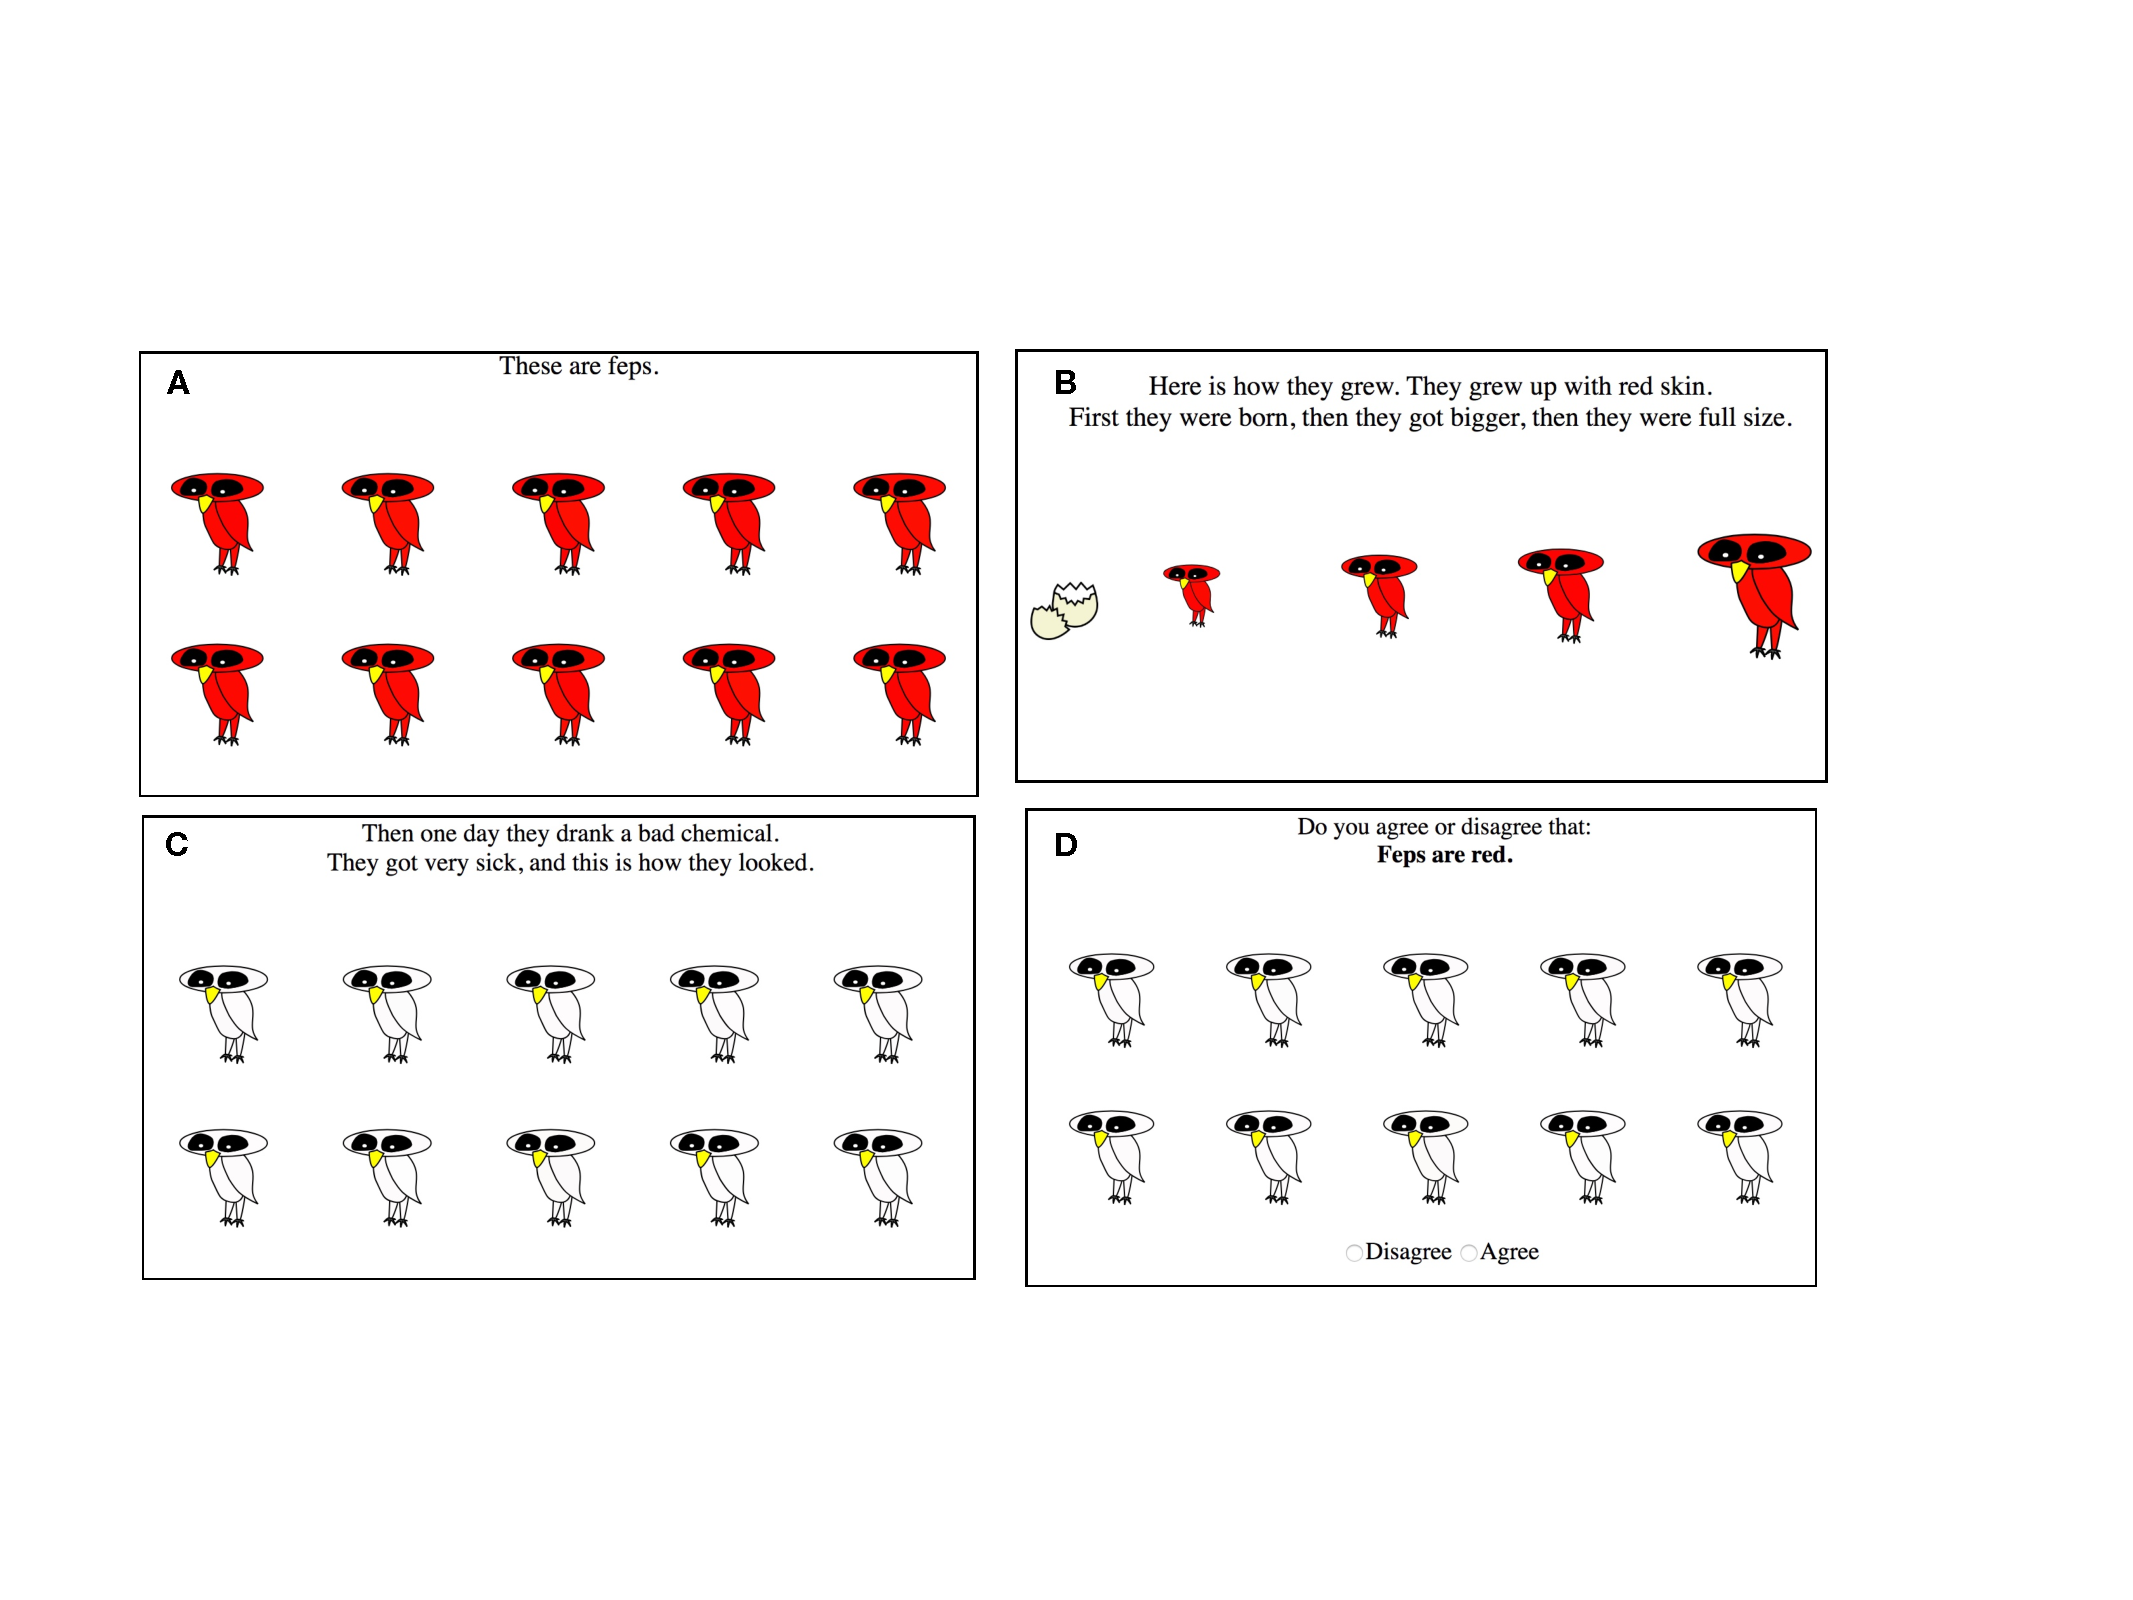
\includegraphics[width=0.8\textwidth]{figs/dobles-expt-fig.pdf}
  \caption{Overview of Expt. 1 (intrinsic origins, property lost condition shown) A: Participants are first introduced to ten identical exemplars of a novel category, either with or without a property (here, shown with the target property of being red). B: The origins of the property are described, either they are born with the property or the acquire it through extrinsic means (born with property shown). C: The event is described and event outcome shown
(here, property is lost). D: Participants evaluate the generic sentence.}
\end{figure}

We hypothesize that the impact of conceptual information on generic language is mediated by participants' expectations about the property. \citeA{Tessler2019} found that it was participants' frequency beliefs about the future that mattered for endorsing habitual sentences (another linguistic expression that conveys generalization) like \emph{John runs} and not the objective, past frequency. 
To test this hypothesis, we collected judgments from a separate group of participants ($n = 80$) about the probability that a future instance of the category (e.g., a doble born today) would grow up to have the property (have claws).
We find similar main effects on the predicative probability judgments  property origins (intrinsic > extrinsic origins; \betaCI{brm_doblesPrev_2way_randInt-subj-proptype.csv}{originsintrinsic} and maintained > lost outcome;  \betaCI{brm_doblesPrev_2way_randInt-subj-proptype.csv}{event_outcomemaintained}) and that that the mean predicted prevalence judgments strongly predict the generic endorsement results ($r = \rlgetnum{expt1_prev_gen_correlations.csv}{condition}{fourConditions}{correlation}{2}$).
We additionally find by-item variability (color features vs. body part features) that is strongly correlated between the two measures  ($r = \rlgetnum{expt1_prev_gen_correlations.csv}{condition}{byItem}{correlation}{2}$). 
Thus, beliefs about property origins influences generic endorsement via influencing beliefs about future prevalence. 




The fact that participants were sensitive to the outcome of the event when endorsing the generic suggests that their beliefs about the stability of these properties influenced their judgments.
For example, participants may believe that the fact that the property can be lost based on drinking a chemical indicates that the property is relatively unstable feature, analogous to heads of hair on adult male humans.
Similarly, the existence of properties in the environment that individuals can come across and acquire is perhaps some evidence that the this external cause of the property is relatively stable \red{(cite Nadya V's work)}.. 
The exploratory analysis is consistent with this if participants believe skin color to be a less malleable property than the body part stimuli.

\subsection{Experiment 2: Dangerousness}


\citeA{Leslie2007} brings our attention to examples like the following:

\begin{enumerate}
\item Sharks attack bathers.
\item Rottweilers maul children. 
\item Mosquitos carry the West Nile Virus.
\end{enumerate}

\noindent arguing that these generic statements are reasonable utterances by virtue of the fact that the ``the property in question is the sort of property of which one would be well served to be forewarned, even if there were only a small chance of encountering it'' (Leslie, 2008; p.15).
(\citeA{Leslie2008} further goes on to speculate that one mediator of dangerous knowledge on generic endorsement is the property's projectibility, or a speaker's perception of the prevalence of the feature \cite{Rothbart1978}.)
Consistent with this intuition,  \citeA{Cimpian2010} (Expts. 1\&4) found that generics about novel categories (e.g., "Lorches have purple feathers") are endorsed more highly when the property is distinctive (\emph{distinctive purple feathers}) or dangerous (\emph{dangerous purple feathers}).
We replicated the original findings by \citeA{Cimpian2010} that these generics are specifically endorsed more at low levels of prevalence (e.g., when only 30\% have the feature; $n=80$; original $n=15$). 
Describing properties as either dangerous or distinctive yields a different pattern of endorsements than when properties are not described as such, which manifests as endorsements exhibiting less of a sensitivity to the actual prevalence owing to the fact that generics about these kinds of properties are endorsed more strongly specifically at low prevalence levels, making their endorsement curves more flat \red{(regression model results)}. 

We hypothesize that the impact of dangerousness on generic language results from participants' implicitly construing dangerous properties as distinctive properties. 
For example, \citeA{Tessler2019} showed how truth judgments for ``Mosquitos carry West Nile Virus'' (which is attested to be true, despite the prevalence of carrying West Nile among mosquitos being low) can be accounted for by virtue of the fact that most animals do not carry the West Nile Virus and even among those animals that could carry the virus, the prevalence would be expected to be low (technically: the prevalence prior distribution for the property \emph{carries West Nile Virus} is strongly biased towards low or 0\% prevalence values) \red{(should have a figure showing this... in fact, a figure for both model-based explanations would be good)}. 
To test this, we ran a \emph{prior elicitation study} where we collected participants' beliefs about the statistical distribution of the property, given either dangerous or distinctive (or no) information about the property. 
Specifically, participants ($n=80$) were asked to predict how many different species of animals they thought would have the property as well as to estimate the property's projectibility (given that at least one instance of the category has the property, how many other instances have the property); both of these constructs contribute to the prevalence prior distribution, which impacts participants' endorsements of generics.
The results are shown in \red{Figure}; consistent with our predictions, both distinctive properties \red{regression results)} and dangerous properties (\red{regression results)} were expected to be present in fewer categories in comparison to the control condition (i.e., properties present without any further information). 
At the same time, neither dangerous nor distinctive properties were more projectible than control properties, contra \citeA{Leslie2008}'s speculation. 
Thus, dangerous properties are construed as distinctive properties, which have different generic endorsement profiles for purely statistical considerations. 

As a further test of the explanatory power of these elicited prevalence priors, we incorporating these prior measurements into the computational model of generic endorsement proposed by \cite{Tessler2019}.
\red{Figure} shows that the model is able to accommodate the qualitative effects of dangerousness and distinctiveness on generic endorsement and provide a high degree quantitative fit to the endorsement task data. 
\mht{control models... projectibility alone? or mediation analysis?}


\section{Discussion}

Much of what we learn about the world comes not from direct experience, but from information conveyed to us by others, often in the form of linguistic expressions \cite{Henrich2015, boyd1988culture} . 
The premier case study of abstract knowledge transmission comes in the form of generic language, or generics, which communicate generalizations about categories \cite{Carlson1977, Gelman2009, Rhodes2012}.
Decades of research into generics has illuminated that generics exhibit a complex sensitivity to content and context that has made it near impossible to describe what is common to all generics \cite{Carlson1995, Leslie2007, Sterken2015, Nickel2016, Cohen1999}.
Instead, interest has turned to classifying different kinds of generic sentences and how these might link up to various domain-specific knowledge sources \cite{Prasada2013, Cimpian2010, Gelman2007, tasimi2017differences}.
%\red{(cite prasada, cimpian, tasimi, gelmanbloom, ...)}.
But insofar as there is a thing called a generic sentence, there must be something common to them. 
Here we explore how various domain specific knowledge sources interact with the semantics of generics to influence how people judge generics as true or false. 

How does conceptual knowledge influence our understanding of generics? 
It has been argued that generics are the mind's way of giving voice to primitive conceptual generalizations, and there are several distinct and irreducible criteria that would grant a true generic claim \cite{Leslie2007}.
Here we show that two empirical demonstrations of conceptual knowledge moderating understanding of generics can be explained in terms of more basic, probabilistic knowledge representations. 
The knowledge that members of a category are born with a property \cite{Gelman2007} leads to stronger projectibility to other, future members of the category, in comparison to properties that are acquired through experience.
This stronger projectibility interfaces with a simple, prevalence-based semantics, resulting in increased endorsements.
Dangerous properties \cite{Cimpian2010}, we show, are also less likely to be present in many categories, which results in distributional expectations similar to those of distinctive properties. 
These statistical representations are sufficient to explain the influence of these conceptual moderators on generic endorsements. 

In our examination of the influence of property origins on generic sentences, we found that property origins influenced the projectibility of the property into future instances of the category. 
The notion that generics require examining \emph{sufficiently long histories} has been described before \cite{Cohen1999}, but there is little empirical evidence to support the explanatory power of this construct. 
%In pilot work, we found that a number of similar questions one could ask about projectibility did not all lead to the patterns found in our main experiment. 
In our experiment, we asked \emph{if a new doble were born today, when they grew up}, how likely would they be to have the property?
In pilot work, we asked three similar questions ($n=15$ for each): \emph{If you were to encounter another doble, how likely would they be to have the property?}, \emph{There are 100 other dobles on the planet, how many have the property?}, and \emph{There is another set of dobles on the other side of planet, how many of them have the property?}.
Neither of these questions resulted in the projectibility patterns we saw for the \emph{new doble born today} question. 
This suggests that the notion of \emph{predictive prevalence} has to do with simulating a very close causal history (i.e., not the dobles on the other side of the planet) in full (i.e., simulate ontogeny starting today). 
This interpretation also brings parsimony to a related finding that found participants willing to endorse generics about properties present in only a minority of the category when that minority were adults and the majority babies \cite{Cimpian2010theory}.
These notions may also relate to what it means to be a normal member of the category, what it means to be a \emph{normal doble|} \cite{Nickel2008}.

Our work calls into question the empirical evidence claiming to support the special status of dangerous information on generic language \cite{Leslie2008, Cimpian2010}.
Rather, we deem the question an open empirical one. 
We found that the evidence that has been offered so far is confounded with simpler statistical mechanisms. 
However, the free form explanations of at least a few participants suggests that intuition of utility of conveying dangerous information is present. 
One wrote: ``I decided that I would rather assume all are dangerous than risk injury/death from the chance I come into contact with the species.''
Another: ``The guidelines that came naturally to me were these: I only called a generalization true if it was at least 80-90\% true. However, I always called the generalizations true whenever I thought that doing so would protect people (i.e., such and such animal has dangerous properties), even when they were only 10% true.''
These intuitions suggest that other utility information is entering into the endorsement patterns. 

Our model could be supplemented with these additional utility constraints \cite{Goodman2016, Yoon2016}, but we do not find empirical for that such an alternative is necessary at present to account for the data.
The intuitions shared by some participants are not shared by all: ``I did answer false to all of the questions because everything was under 100\%. A definitive statement like ``Clobs have dangerous yellow fur'' cannot be made for a 90\% average because there are still that 10\%.'' or ``I tried to stick with saying true when the percentage was 90\% because then you can usually make a generalization that all of them have the feature.''
The analysis we provide describes what a strong future test for the \emph{dangerousness} hypothesis would look like: controlling for the impact of dangerous information on the prevalence priors, and measuring the corresponding projectibility of the property, does dangerous information still lead to an increase in endorsement?



\section{Methods}

\subsection{Experiment 1}

\subsection{Experiment 2}

Participants were presented with an evidence statement describing the prevalence of the property within the category as well as highlighting either the dangerousness or distinctiveness of the feature (e.g., ``30\% of lorches have \{dangerous, distinctive, \emph{null}\} purple feathers.''), followed up by another sentence reinforcing the the dangerousness or distinctiveness of the property (e.g., ``These feathers are as sharp as needles and can easily get lodged in you, causing massive bleeding.''; ``No other animals on this island have wide, smooth feathers like these.''). Control items were followed with additional, irrelevant descriptions (e.g., ``These feathers are wide and very smooth to the touch.''). 

%This is confirmed by a Bayesian Bernoulli regression model with fixed-effects of property type (dangerous vs. distinctive vs. neither), prevalence levels (treated as a continuous variable, centered and scaled), and their interaction.
%As well, the model included random intercepts and effects of property type, by participant and by item. 
%We find evidence for different slopes such that both dangerous properties ($\beta_{dangerous\times prevalence}=$ `r format_regression_effects(brms.endorsement.bern.2.summary, "stim_typedanger:prev_centered")`) and distinctive properties ($\beta_{distinctive\times prevalence}=$ `r format_regression_effects(brms.endorsement.bern.2.summary, "stim_typedistinct:prev_centered")`) show less of an effect of prevalence on their endorsement; this is because they are endorsed higher specifically at low prevalence levels, thus making their endorsement curves more flat. 


%Finally, we perform a Bayesian mediation analysis, finding that probabilistic knowledge fully mediates the effects of dangerous information on generic endorsements.
%These results call into question claims about the special status of dangerous information on generic language understanding and suggest more careful experimental controls for future investigations.

%Following our treatment of the priors for novel generics (Ch. 1 Expt. 1, Ch. 3 Expt. 1), we used a zero-inflated beta distribution shape for the prevalence priors, taking the first prior elicitation question (*number of categories*) as the estimate of the probability mass at 0% prevalence and responses to the second prior elicitation question (*projectibility*) as samples from the Beta distribution.


\bibliographystyle{apacite}

\setlength{\bibleftmargin}{.125in}
\setlength{\bibindent}{-\bibleftmargin}

\bibliography{generics}


\end{document}


\end{document}